\documentclass{report}

\usepackage[latin1]{inputenc}    
\usepackage[T1]{fontenc}
\usepackage[francais]{babel}
\usepackage[top=4cm, bottom=4cm, left=2cm, right=2cm]{geometry}


\title{Charte graphique}
\author{Alexandre \bsc{SCHANNE}}
\date{27 Septembre 2016}
\usepackage{graphicx}
\begin{document}
\maketitle
\pagestyle{plain}
\part{Introduction :}
			Cette charte graphique a pour objectif de d�finir et expliquer les diff�rents choix de conception visuel du site internet "<http://s647394915.onlinehome.fr/">. Les d�cisions prises ont un impact sur l'ensemble du site et sur la vision des citoyens de la ville de Thionville et alentours. Ainsi, il est bon de rappeler que les d�cisions furent r�fl�chies en collaboration entre la mairie de Thionville et l'entreprise "<...">, r�sponsable de la conception et la distribution du site web.\\
			
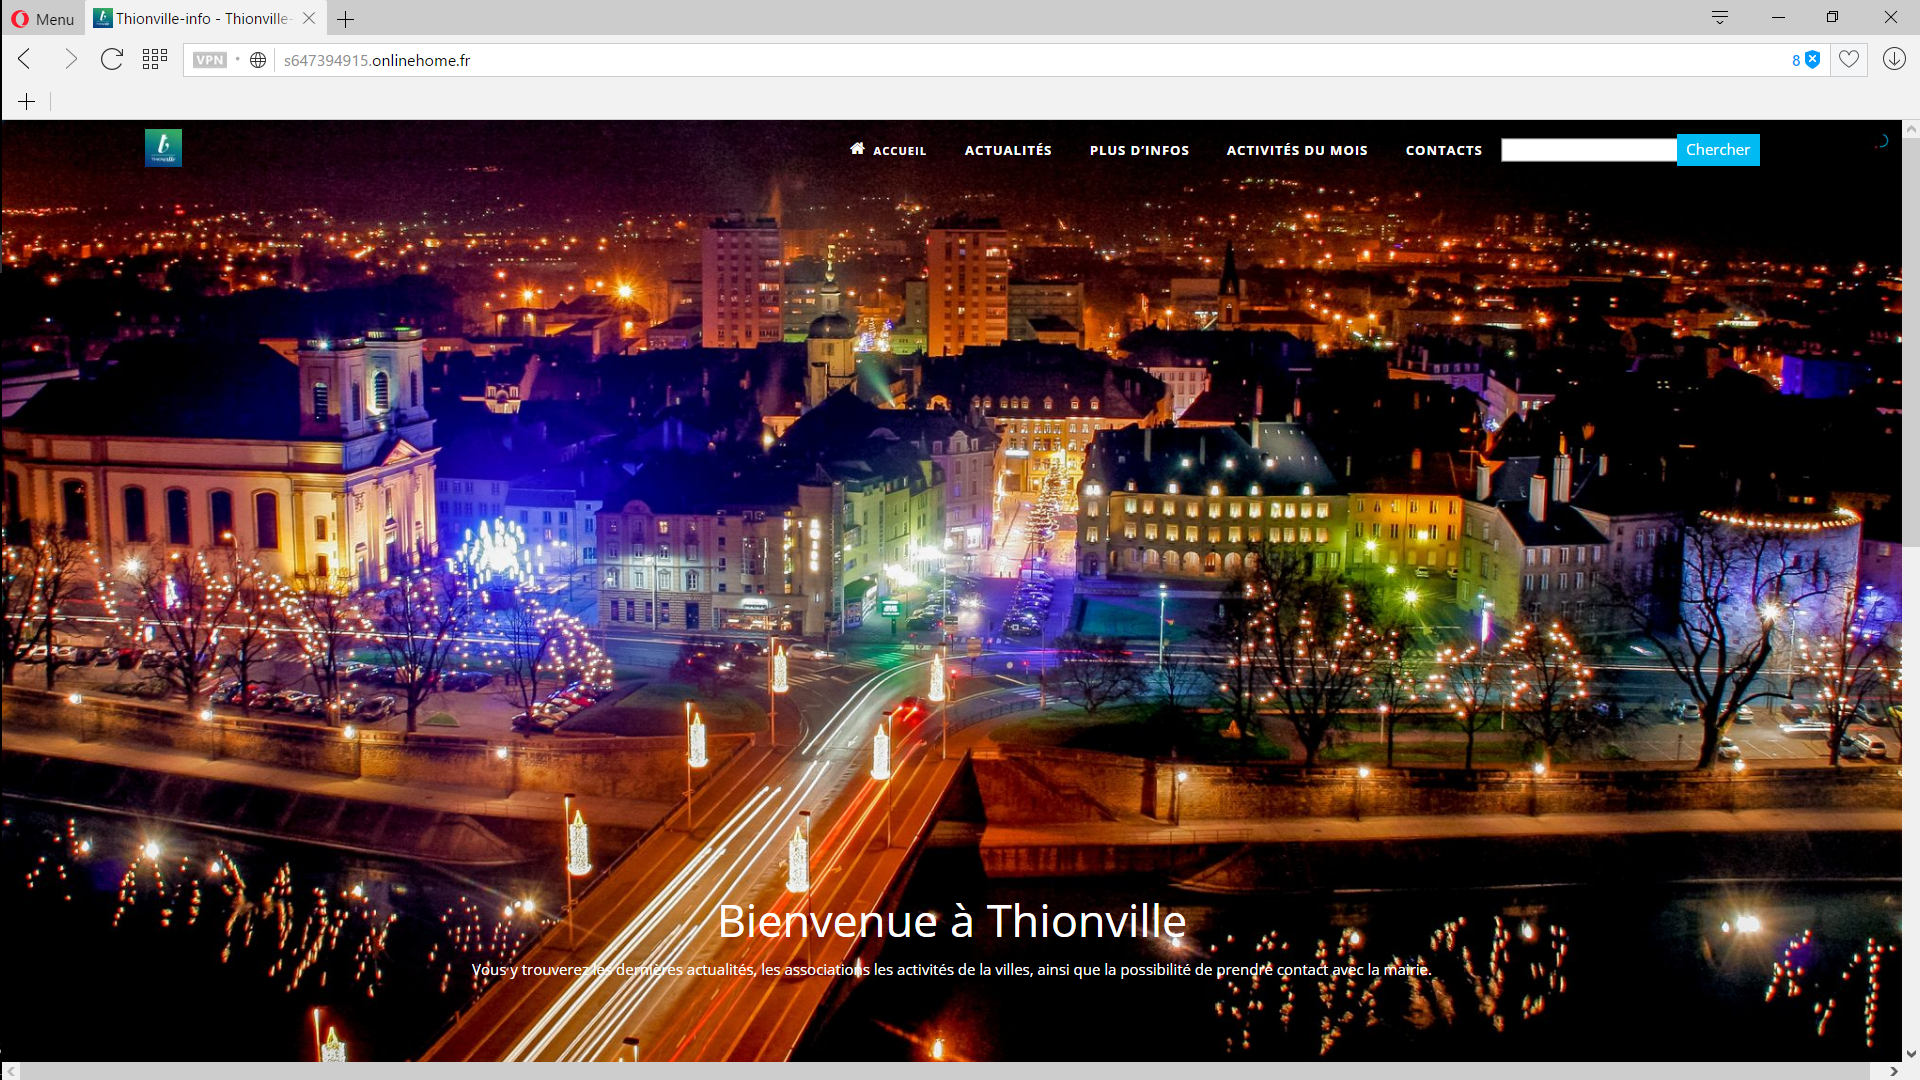
\includegraphics[scale=0.38]{ThionvilleNuit.png}

\part{Le choix des formes et des couleurs :}
\chapter{Les couleurs :}
			Pour soigner le message que nous voulions transmettre, les couleurs se portent essentiellement sur le noir et le bleu clair : (\#bee2e2, couleur en hexad�cimal). L'objectif �tant double :
\begin{itemize}
\item La couleur fonc�e reflette l'activit� nocturne de la ville, toujours riche. Les terrasses, les promenades au bord de l'eau, fl�ner en ville et les restaurants sont des activit�s fortes que l'on voulait mettre en valeur.//
En terme de couleur, l'image de la page principale est essentiellement sombre avec des couleurs chaudes, la cible est donc les jeunes pour montrer le potentiel de la ville.
\item La partie claire du site, que l'on retrouve sur l'ensemble des pages est volontairement p�le. Il est important que les visiteurs du site web n'aient pas les yeux attaqu�s par une couleur trop vive. Le bleu reflette le jour et les activit�s qui y sont li�es.
\end{itemize}
On a donc un jeu de 2 couleurs, fondamental pour laisser deux ambiances diff�rentes en fonction de l'information que l'on est venu chercher.\\

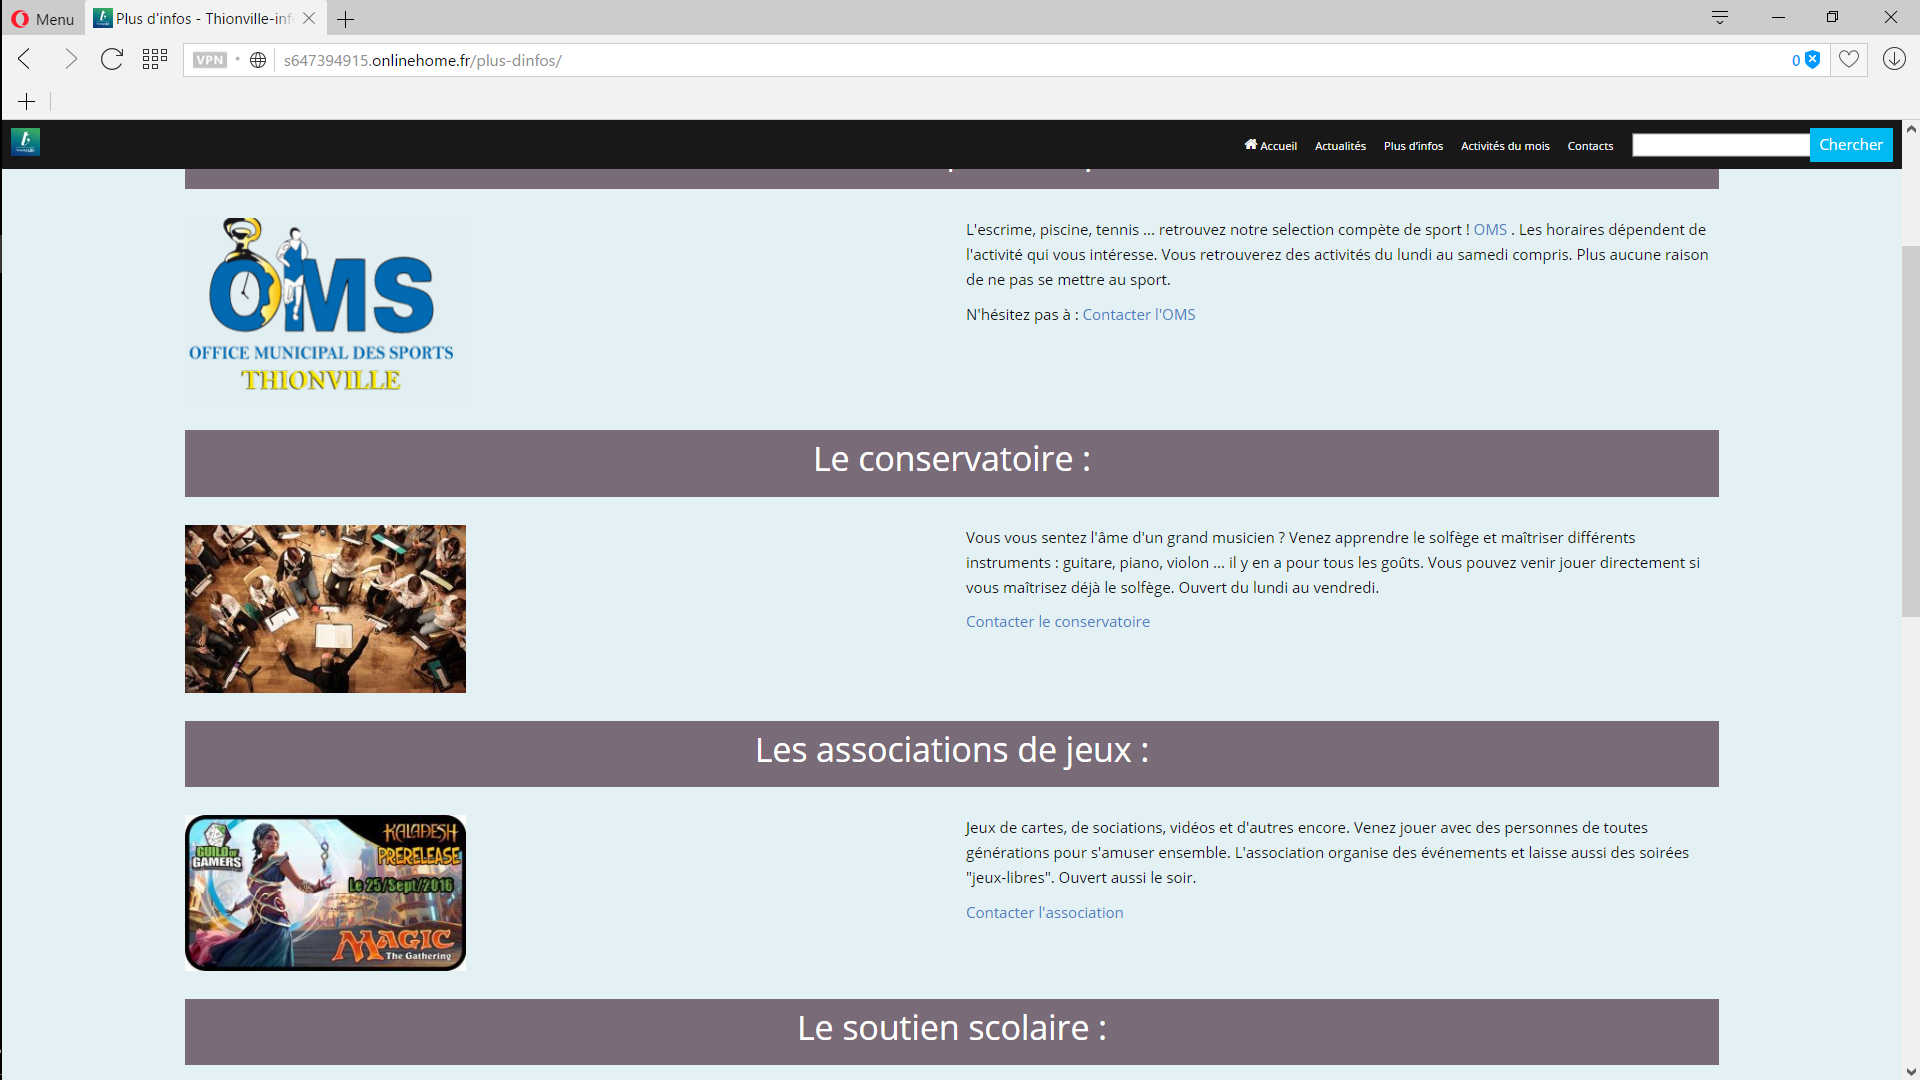
\includegraphics[scale=0.38]{ThionvilleBleu.png}

\chapter{Les formes :}
\section{Moderne :}
			Un site "<moderne">, diff�rent des site disposants d'une explosion d'article dans tous les sens, dans lequel chaque page est bien d�finie. Un style rectangulaire acompagnera les visiteurs sur l'ensemble du site pour obtenir une architecture contemporaine.
\section{Adapt� :}
			Du fait de l'accroissement explosif des appareils portatifs, la responsivit� du site est une notion crutiale pour que tout utilisateur puisse naviguer confortablement. Ainsi, nous avons fait les choix suivant :
\begin{itemize}
	\item L'image de la page principale est conserv�e m�me en cas d'�cran plus petit, pour ne pas regarder un site "<sans vie">.
	\item Les �l�ments sont positionn�s en ligne de haut en bas, pour que la diff�rence d'affichage entre divers �crans soit le moins visible possible. L'architecture n'est donc pas modifi�e en fonction de son �cran.
\end{itemize}}



\end{document}
